

\documentclass[../../main.tex]{subfiles}



\graphicspath{ {imagenes/} }

\begin{document}
\section{OpAmp}
\subsection{Introducci\'on}
Se analizaron dos circuitos con Amplificadores operacionales. El primero es un circuito inversor, cuya salida es opuesta a la entrada y  la aplifica o atenua, de a cuerdo a como se configure. El segundo es no inversor, igual que el primero, atenua o amplifica la señal de entrada, pero no la invierte.
El objetivo es evaluar las caracteristicas lineales y no lineales de los amplificadores operacionales. Tambien la respuesta en frecuencia y la respuesta  distintos valores de tensiones de entrada.


\subsection{Circuito inversor}
\todo{algo desir alog}


\begin{figure}[H]
\centering

\begin{circuitikz}[scale=1]
\def\xspacing{2}
\def\xstart{0}
\def\yspacing{2}	
\def\ystart{0}

%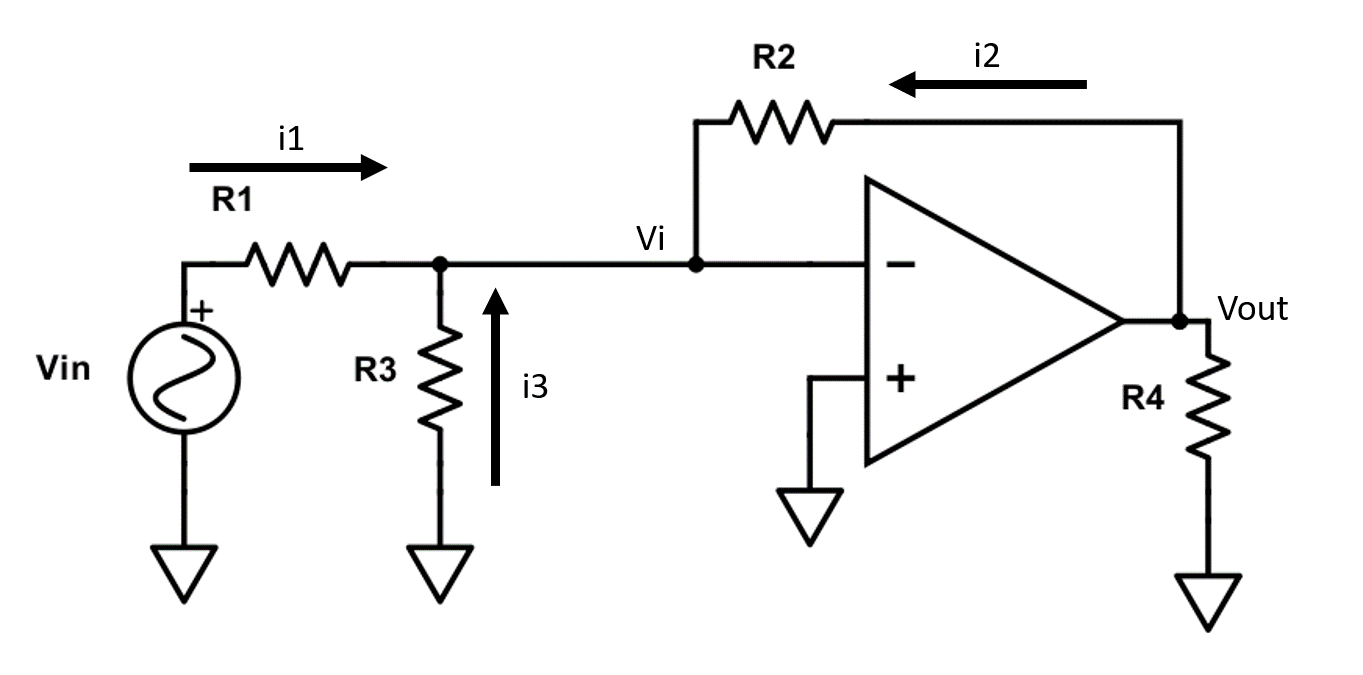
\includegraphics[width=0.5\textwidth]{imagenes/xxx.png}




%dibujo malla izquierda
\draw   						(\xstart, \ystart) node[ground]{}
		to [vsourcesin]	 	(\xstart, \ystart + \yspacing)
		to [R=$R_1$, i>^=$i_1$] (\xstart + \xspacing, \ystart + \yspacing)
		to [R=$R_3$, i<^=$i_3$] (\xstart + \xspacing, \ystart)
		to (\xstart + \xspacing, \ystart) node[ground]{}

%dibujo opamp
%el opamp tiene la misma altura que scale, y las patitas - y + estan en .25*scale y .75*scale
%nos queda - en ystart+yspacing y + en ystart+spacing-0.5

		(\xstart + 3*\xspacing, \ystart + \yspacing - .5) node[op amp] (opamp) {}

%dibujo conexiones a opamp
	 						   (\xstart + \xspacing, \ystart + \yspacing)
		to [short]			  (opamp.-)
								(opamp.+)
		to [short]			  ($(opamp.+)+(0,-\yspacing + 1)$) node[ground]{}	%se me va la patita
								(\xstart + 2*\xspacing, \ystart + 1*\yspacing)
		to [short, *-]		  (\xstart + 2*\xspacing, \ystart + 1.7*\yspacing)
		to [R=$R_2$, i<^=$i_2$] (\xstart + 4*\xspacing, \ystart + 1.7*\yspacing)
		to [short, -*]		  (\xstart + 4*\xspacing, \ystart + 1*\yspacing -.5)
		to [short]			  (opamp.out)
								(\xstart + 4*\xspacing, \ystart + 1*\yspacing -.5)
		to [R=$R_4$]			(\xstart + 4*\xspacing, \ystart) node[ground]{};


\end{circuitikz}


\caption{Esquematico del circuito Inversor}
\end{figure}

Los valores de las resistencias utilizados fueron los indicados en la Tabla \ref{tab=vResistencias}.

\begin{table}[h]
\begin{center}
\begin{tabular}{|l|l|l|l|}
\hline
Caso & $R_{1}=R_{3}$ & $R_{2}$ & $R_{4}$\\
\hline \hline
1 & $5 K\Omega $ &  $50 K\Omega $ &  $20 K\Omega $ \\ \hline
2 & $5 K\Omega $ &  $5 K\Omega $ &  $20 K\Omega $ \\ \hline
3 & $50 K\Omega $ &  $5 K\Omega $ &  $100 K\Omega $ \\ \hline
\end{tabular}
\caption{Valores de resistensias.} 
\label{tab=vResistencias}
\end{center}
\end{table}



\subsubsection{Caso $A_{vol}$ infinito}

Como $A_{vol}$ lo consideramos infinito, $V_{i}=0$ \big( tierra virtual \big).Por ende $i_{3}=0$ e $i_{2}=-i_{1}$, Ademas no circula corriente por la entrada del   amplificador operacional.
\begin{gather}
V_{out}=-\frac{i_{1}}{R_{2}}\label{eq=CircuitoA6}\\
i_{1}=\frac{V_{in}}{R_{1}}\label{eq=CircuitoA7}
\end{gather}
Reemplazando \ref{eq=CircuitoA7} en \ref{eq=CircuitoA6} y operando algebraicamente se obtine:
\begin{equation}
\frac{V_{out}}{V_{in}}= -\frac{R_{2}}{R_{1}} \label{eq=CircuitoAideal}
\end{equation}


\subsubsection{Caso $A_{vol}$ finito}

Como $A_{vol}$  lo consideramos finito, $V^{+}\neq V^{-}$ . Se considera que no circula corriente por  los terminales de entrada del amplificador operacional, devido a la alta impedancia que hay entre ellos.

\begin{gather}
V_{out}= -V_{i}\cdot A_{vol}\label{eq=CircuitoA1}\\
i_{1}=\frac{V_{in}-V{i}}{R_{1}}\label{eq=CircuitoA2}\\
i_{2}=\frac{V_{out}-V_{i}}{R_{2}}\label{eq=CircuitoA3}\\
i_{3}=\frac{-V_{i}}{R_{3}}\label{eq=CircuitoA4}\\
i_{1}+i_{2}+i_{3}=0\label{eq=CircuitoA5}
\end{gather}

Reemplazando \ref{eq=CircuitoA1},\ref{eq=CircuitoA2},\ref{eq=CircuitoA3},\ref{eq=CircuitoA4} en \ref{eq=CircuitoA5}, se obtiene:


$$\frac{V_{in}}{R_{1}} + \frac{V_{out}}{R_{2}}+\frac{V_{out}}{A_{vol}}\cdot \bigg( \frac{1}{R_{1}} + \frac{1}{R_{2}} + \frac{1}{R_{3}} \bigg) = 0$$

Operando algebraicamente, se obtiene:

\begin{equation}
\frac{V_{out}}{V_{in}}= - \frac{A_{vol} \cdot R_{2} \cdot R_{3}}{A_{vol}\cdot R_{1} \cdot R_{3} + R_{2} \cdot R_{3} +  R_{1} \cdot R_{3} + R_{1} \cdot R_{2} }\label{eq=gananciaAfinito}
\end{equation}
Observacion

$$ \lim_{A_{vol}\to\infty} \big( \ref{eq=gananciaAfinito} \big) = -\frac{R_{2}}{R_{1}} $$
La expresion se redujo a la ganancia del circuito, con el apmlificador operacional ideal\\ \big(\ref{eq=CircuitoAideal}\big).

\subsubsection{Caso $A_{vol}$  con polo dominante}

\begin{equation}
A_{vol }=\frac{A_{0}}{1+\frac{s}{W_{p}}}\label{eq=AvolWp}\\
\end{equation} 

Reemplazando \big(\ref{eq=AvolWp}\big) en  \big(\ref{eq=gananciaAfinito}\big)  se obtiene:

\begin{equation}
\frac{V_{out}}{V_{in}}= - \frac{\frac{A_{0}}{1+\frac{s}{W_{p}}} \cdot R_{2} \cdot R_{3}}{\frac{A_{0}}{1+\frac{s}{W_{p}}}\cdot R_{1} \cdot R_{3} + R_{2} \cdot R_{3} +  R_{1} \cdot R_{3} + R_{1} \cdot R_{2} }
\end{equation}

Llamando $K= R_{2} \cdot R_{3} +  R_{1} \cdot R_{3} + R_{1} \cdot R_{2}$


\begin{equation}
\frac{V_{out}}{V_{in}}=- \frac{A_{0} \cdot  R_{2} \cdot  R_{3} }{A_{0} \cdot R_{1} \cdot  R_{3} + K }  \cdot \frac{1}{1 +\frac {S}{\frac{W_{p}  \cdot \big( A_{0} \cdot R_{1} \cdot R_{3} + K \big) }{K}}} \label{eq=poloDominante}
\end{equation}

 Despejando se obtiene la frecuencia de corte del circuito:
\begin{equation}
f_{P}=\left( \frac {A_{0} \cdot R_{1} \cdot R_{3} + K}{K}\right)  \cdot \frac{W_{P}}{2\cdot \pi}  \label{eq=fCorte}
\end{equation}

\textit{Observacion:}  la ecuacion \big(\ref{eq=poloDominante} \big) posee la misma forma que la funcion transferencia de un pasabajos.



El amplificador operacional utilizado fue el LM324 de ON Semiconductor, de la hoja de datos se obtuvieron las siguientes cararacteristicas del integrado:


\begin{table}[h]
\begin{center}
\begin{tabular}{|l|l|}
\hline
$A_{0}$ & $f_{P}$ \\
\hline \hline
$10\cdot 10^{4}$& $ 12Hz $ \\ \hline

\end{tabular}
\caption{Caracteristicas del LM324} 
\label{tab=lm324Carac}
\end{center}
\end{table}
Donde $A_{0}$ es la ganancia del amplificador operacional a lazo abierto y  $f_{P}$ es la frecuencia de corte a lazo abierto. A partir de las tablas \ref{tab=vResistencias} y \ref{tab=lm324Carac} y de ecuación  \ref{eq=poloDominante}, se calcularon las caracteristicas de las tres configuraciones del circuito analizadas.

\begin{table}[h]
\begin{center}
\begin{tabular}{|l|l|l|l|}
\hline
Caso &Ganancia ideal & Ganancia $A_{vol}$ finito & Frecuencia de corte\\
\hline \hline
1 & $-10$ & -9,997 & 54,7$KHz$ \\ \hline
2 & $-1$ &  $-0,999 $ &  386$KHz$  \\ \hline
3 & $-0,1$ &- 0,099 &960$KHz$\\ \hline
\end{tabular}
\caption{Ganancia y frecuencia de corte del circuito.La ganancias es en veces.} 
\label{tab=gananciayFrecCorte}
\end{center}
\end{table}

Acontinuacion se graficaran los tres casos del circuito inversor, comparando la respuesta en frecuencia con  $A_{vol}$ infinito y $A_{vol}$ con polo dominante.

\begin{figure}[H]
\centering
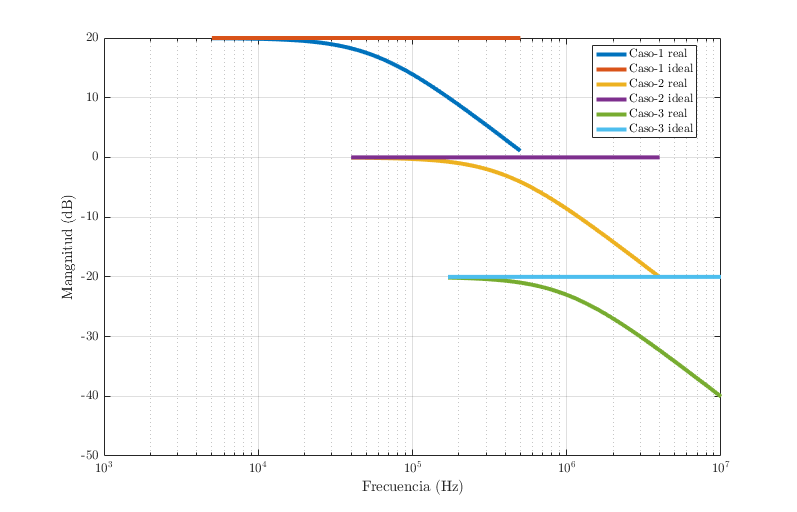
\includegraphics[width=0.8\textwidth]{real_ideal_mag_inv}
\caption{Compración del modulo de la respuesta en frecuencia de los tres casos}
\end{figure}

\todo{poner graficos de fase?}

El error relativo de considerar $A_{vol}$  como infinito, se calculo $ Error(w) = \frac {\mid Ganancia A_{vol}(w) -Ganancia A_{vol} inifinito \mid} {\mid Ganancia A_{vol} (w) \mid }$, de esta manera se obtuvieron los siguientes graficos:

\begin{figure}[H]
\centering
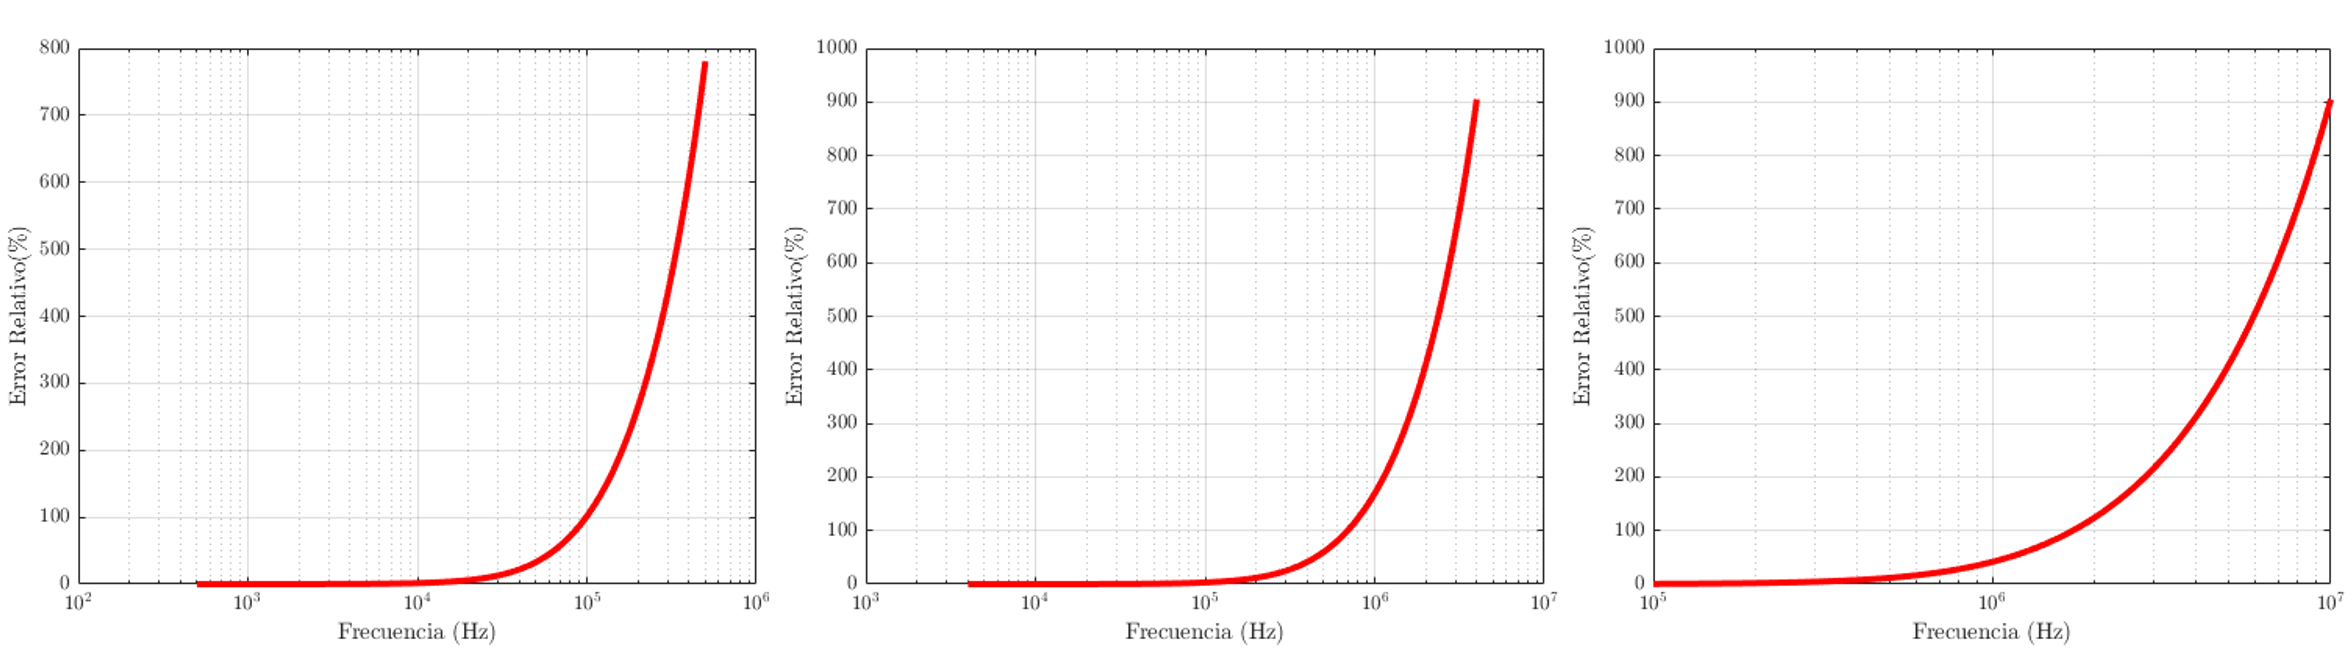
\includegraphics[width=1\textwidth]{error_inv}
\caption{Error relativo porcentual, de izquierda a derecha Caso 1, Caso 2 y Caso 3} \label{fig=errorInv}
\end{figure}


Como se observa en los tres graficos de la figura \ref{fig=errorInv}, el error una decada antes del polo dominante es menor que el 1 \% , por ende utilizando el Amplificador Operacional a una frecuencia menor que una decada antes de la frecuecia de corte, se lo puede considerar como ideal.
\subsubsection{Alinealidades del Amplificador Operacional}
En esta seccion se analizaran las alinealidades del Amplificador operacional
\begin{itemize}  
\item Saturacion, los amplificadores operacionales poseen alimentacion ( $+-V_{cc}$ ) externa para asi poder aplificar. Por ende la salida del amplificador no puede superar a la alimentacion. Si la señal de entrada fuera tal que aplificada superara la alimentacion, el amplificador operacional entrega a la salida $+ o -V_{cc}$. No todos los amplificadores operacionales saturan en $+-V_{cc}$, generalmnete lo hacen por devajo de dichas tensiones y no necesariamente saturan a la misma tension, por ejemplo un Amplificador operacional es alimnetado con +- 10 v, y la saturacion se da a los -8 v y a los 9v. 
\item Slew Rate, es la tasa de cambio de la tension en funcion del tiempo. Los amplificadores Operacionales poseen un slew rate maximo, a partir del cual no pueden seguir la señal de entrada y la salida se distorciona. Para señales senoidales, la relacion entre la frecuencia de entrada, la ganancia y el slew rate es $ SlewRate_{max}=G  \cdot A \cdot 2 \cdot \pi \cdot f $, donde $ G $ es la ganancia del circuito, $ A $ es la amplitud de la señal de entrada y $f$ es la frecuencia de la señal.  
\item Crossover Distortion, los amplificadores operacionales clase b y AB (ejemplo el LM324), poseen la caracteristica que la salida se encuentra en 0 v, cuando la tension de entrada del operacional se encuentra entre -0,7 v y 0,7v.
\end{itemize}

\subsubsection{Dc sweep}
El dc sweep consiste en variar la tensión de entrada (corriente continua) del circuito y observar la salida. En este caso se varió la entrada entre $\pm V_{cc}$($\pm 15 v$). Dicho procedimiento se realizó de la siguiente manera, en la entrada se inyecto una rampa  cuya  tensión variaba entre$\pm V_{cc}$ y de periodo 60 segundos, y la salida se midió con el osciloscopio. Luego se exportaron los datos del osciloscopio en formato CSV y se supepuso la informacion en el siguiente grafico.

\begin{figure}[H]
\centering
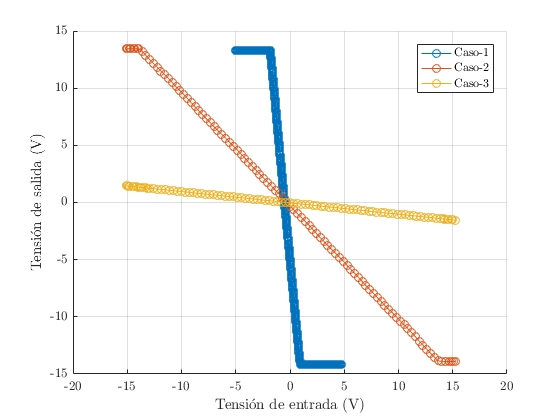
\includegraphics[width=1\textwidth]{dc_sweep_inv}
\caption{Dc Sweep Medido} \label{fig=dcInv}
\end{figure}

\begin{figure}[H]
\centering
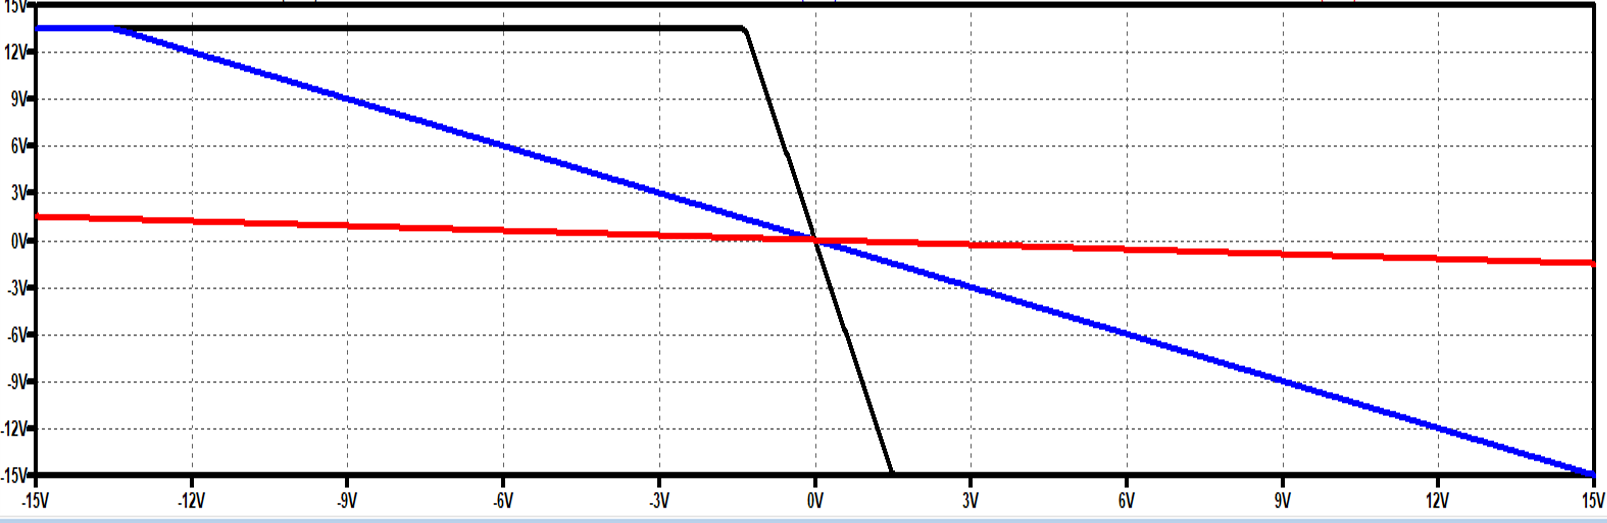
\includegraphics[width=1.1\textwidth]{dc_sweep_inv_sim}
\caption{Dc Sweep Simulado, el grafico negro corresponde al Caso 1, el azul al Caso 2 y el rojo al Caso 3} \label{fig=dcInvSim}
\end{figure}

La figura \ref{fig=dcInv}, es la superposición de los dc sweep medidos de los tres casos. En ella se manifiesta fenómeno de la saturación del amplificador operacional, en dos de los tres casos analizados. Dependiendo de la ganancia del circuito (pendiente de la recta), la saturación se da a distintitas tensiones de entrada, a mayor ganancia (Caso 1) satura a menor tensión que el circuito de menor ganancia (Caso 2). Como se alimentó con $\pm V_{cc}$ el circuito 3 no se logró llegar a la saturación. Para lograrlo se tendría que haber realizado el dc sweep con tensiones del orden de 150 V.
Tanto en la figura \ref{fig=dcInv} como en la figura \ref{fig=dcInvSim},  se observa que la saturación se da a tensiones en módulo menores que VCC. Sin embargo la medición y la simulación no coinciden, esto se puede deber a que el modelo utilizado no se ajusta al amplificador operacional que se usó en el circuito.

\subsubsection{Respuesta en frecuencia}

La ecuación \ref{eq=poloDominante} es la función transferencia del circuito, como la parte real del polo es negativa el sistema es bibo-estable y para hallar la respuesta en frecuencia vasta con reemplazar s=i2pif. El sistema corresponde a un circuito pasa bajos de primer orden, por ende se esperaría que las frecuencias una década menor que la frecuencia de corte no se vean atenuadas y frecuencias una década superiores a la frecuencias de corte, se vean atenuadas. En cuanto a la fase debería variar entre $180^{\circ}$, una década antes de la frecuencia de corte, y$90^{\circ}$ grados una década después de la frecuencia de corte, pasando por los $135^{\circ}$ en la frecuencia de corte.
\\
En la medición de la respuesta en frecuencias se tuvieron que tener en cuenta las alinealidades ya mencionadas. Para que el crossover distortion no afecte las mediciones, a la señal de excitación se la monto sobre una tensión continua, tal que la señal de entrada no cruce por cero. Esto provocó que la amplitud de la señal tenga que ser menor que la esperada para que no se sature la salida. Otro factor importante a tener en cuenta es el slew rate. En base a esto la tensión de entrada quedo limitada de la siguiente manera.

\begin{figure}[H]
\centering
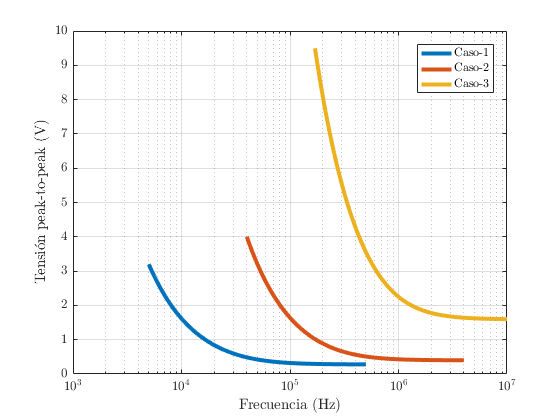
\includegraphics[width=1\textwidth]{slew-rate-inv}
\caption{Tension de entrada,slew rate} \label{fig=srInv}
\end{figure}

El grafico \ref{fig=srInv}, muestra la máxima tensión de entrada en cada caso, sin embargo únicamente tiene en cuenta el slew rate, entonces de acuerdo al offset de la señal se limitara la amplitud para que no haya saturación.
\\
Teniendo en cuenta los factores mencionados se midió la respuesta en frecuencia del circuito.

\begin{figure}[H]
\centering
\begin{subfigure}[http]{0.49\textwidth}
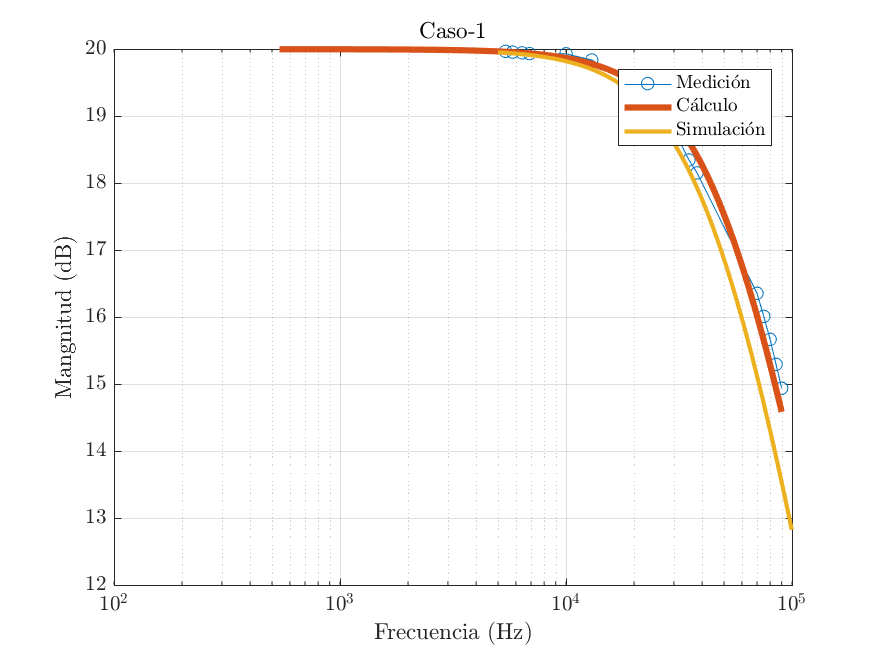
\includegraphics[width=\textwidth]{Caso-1_mag_inv}
\caption{Magnitud}\label{fig=magInvC1}
\end{subfigure}
\begin{subfigure}[http]{0.49\textwidth}
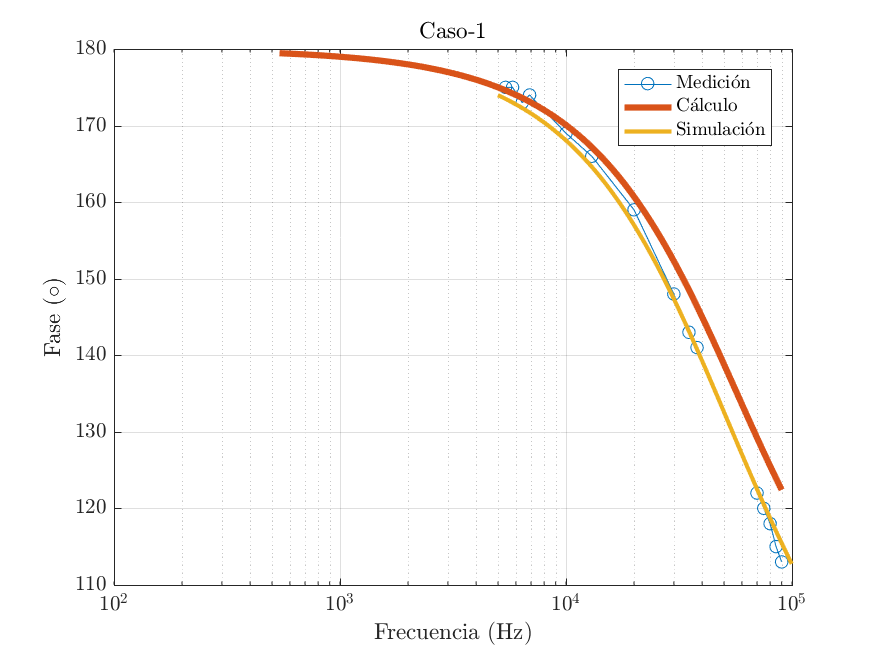
\includegraphics[width=\textwidth]{Caso-1_fase_inv}
\caption{Fase}
\end{subfigure}
\caption{Caso 1 - superposición respuesta en  frecuencia medida, simulada, calculada}
\end{figure}

\begin{figure}[H]
\centering
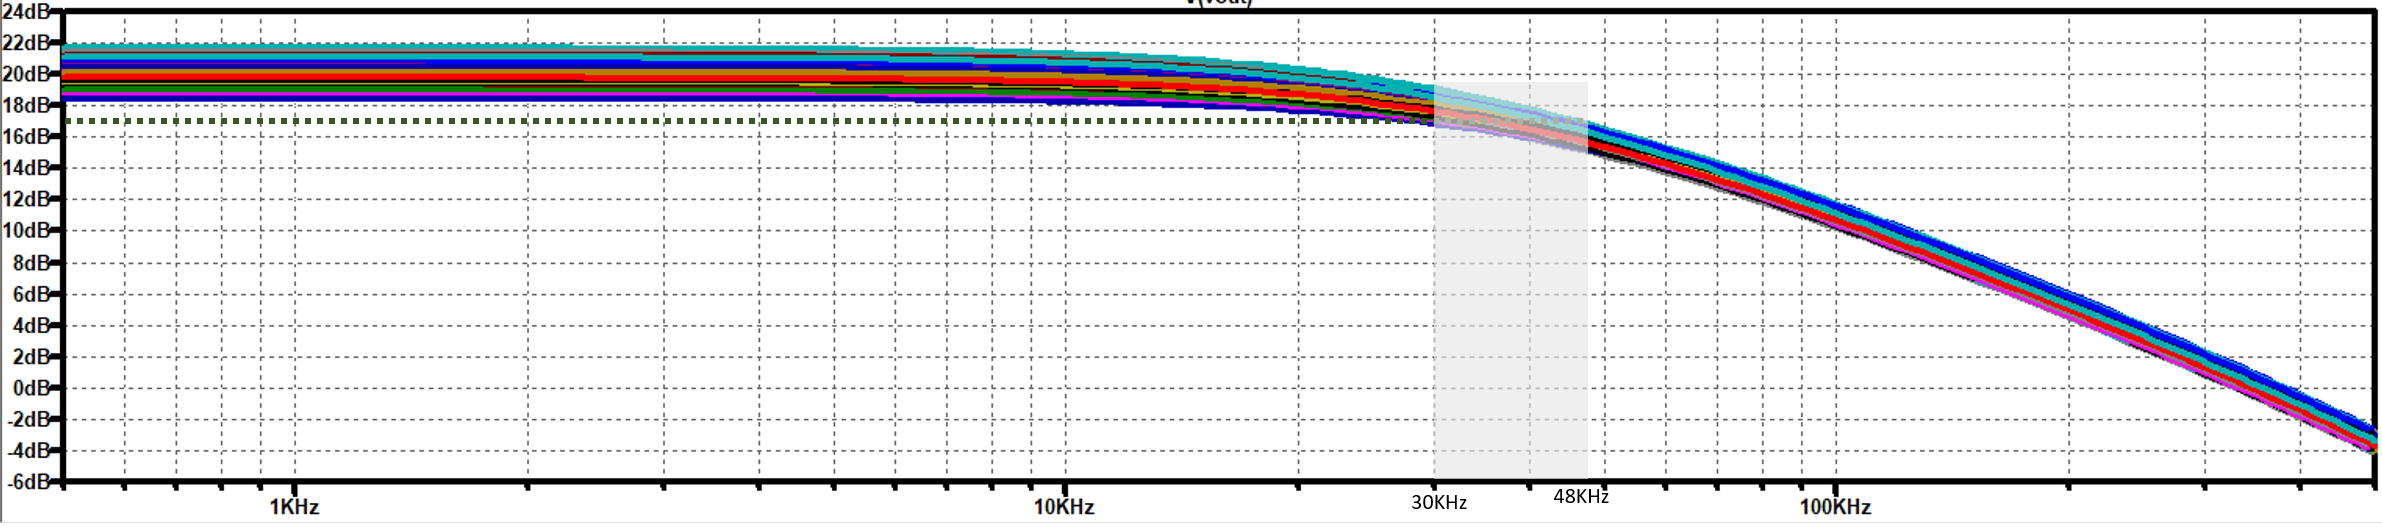
\includegraphics[width=1\textwidth]{montecarlo_inv_c1}
\caption{Montecarlo Caso-1} \label{fig=mcInvC1}
\end{figure}


De la figura \ref{fig=magInvC1}, obtuvimos la frecuencia de corte del circuito,a la cual la caida de la ganancia es de 3dB. Dicha frecuencia de corte es $47KHz$, la cual es distinta a la calculada teoricamente en la tabla \ref{tab=gananciayFrecCorte}. Sin embargo, se puede aceptar dicha frecuencia de corte, devido a que los componentes tienen tolerancias, tal como se observa en el Montecarlo (grafico  \ref{fig=mcInvC1} ) la frecuencia de corte pertenece al intervalo marcado en el grafico.



\begin{figure}[H]
\centering
\begin{subfigure}[http]{0.49\textwidth}
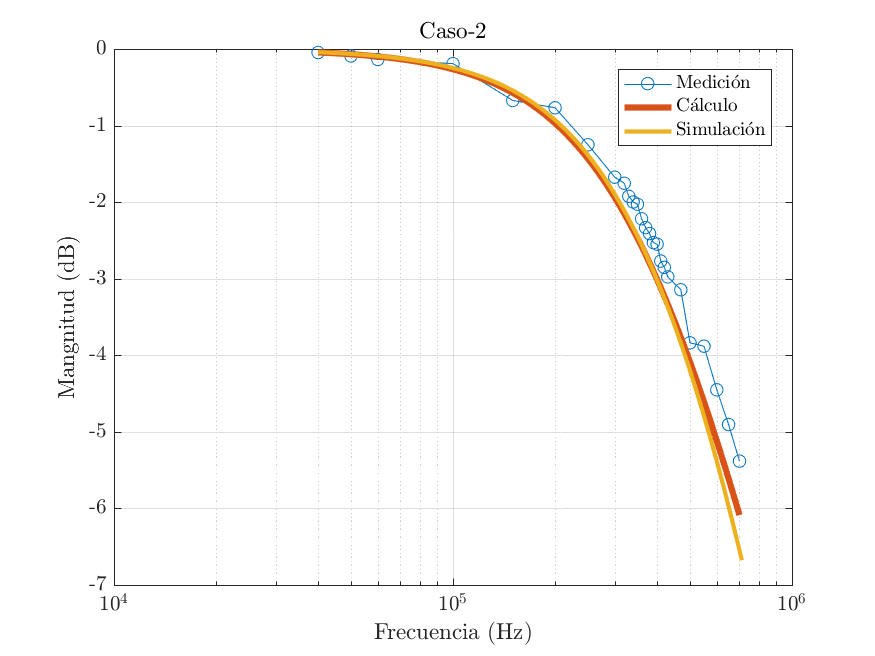
\includegraphics[width=\textwidth]{Caso-2_mag_inv}
\caption{Magnitud}\label{fig=magInvC2}
\end{subfigure}
\begin{subfigure}[http]{0.49\textwidth}
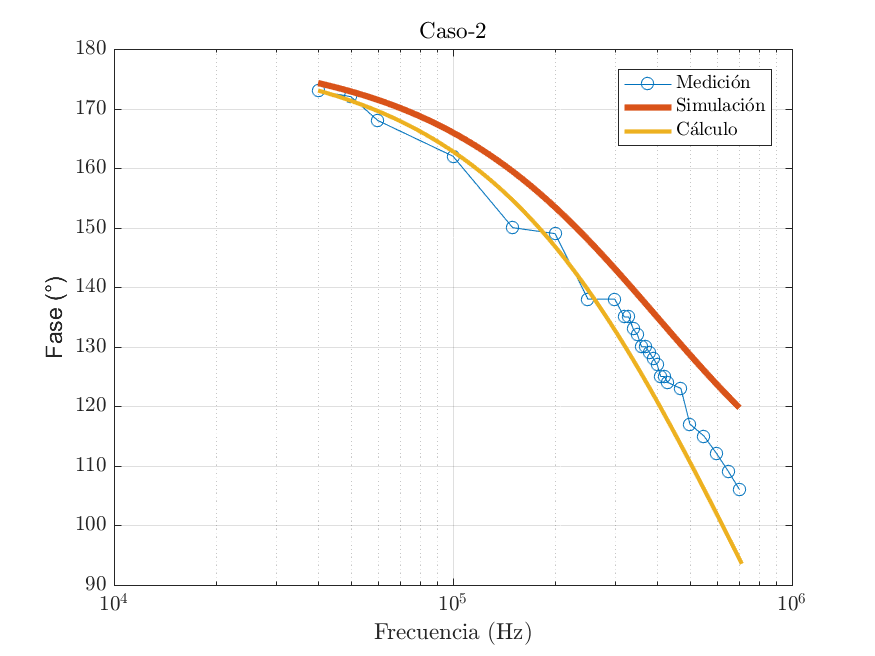
\includegraphics[width=\textwidth]{Caso-2_fase_inv}
\caption{Fase}
\end{subfigure}
\caption{Caso 2 - superposición respuesta en  frecuencia medida, simulada, calculada}
\end{figure}

\begin{figure}[H]
\centering
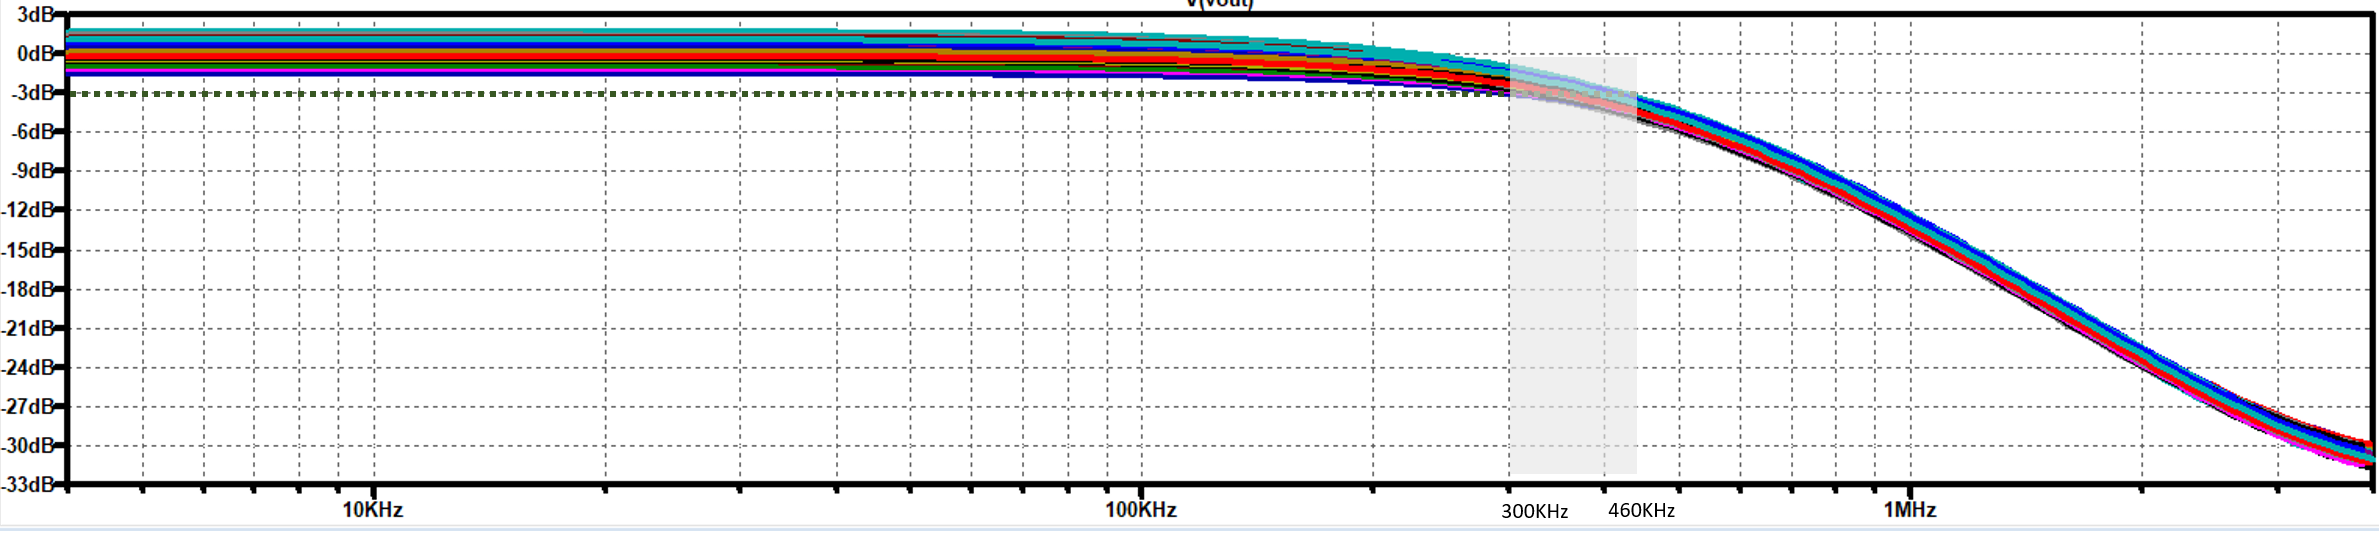
\includegraphics[width=1\textwidth]{montecarlo_inv_c2}
\caption{Montecarlo Caso-2} \label{fig=mcInvC2}
\end{figure}

\todo{desir alguna reflexion mas al respecto}
De la figura \ref{fig=magInvC2}, obtuvimos la frecuencia de corte del circuito,a la cual la caida de la ganancia es de 3dB. Dicha frecuencia de corte es $430KHz$, la cual es distinta a la calculada teoricamente en la tabla \ref{tab=gananciayFrecCorte}. Sin embargo, se puede aceptar dicha frecuencia de corte, devido a que los componentes tienen tolerancias, tal como se observa en el Montecarlo (grafico  \ref{fig=mcInvC2} ) la frecuencia de corte pertenece al intervalo marcado en el grafico.

\begin{figure}[H]
\centering
\begin{subfigure}[http]{0.49\textwidth}
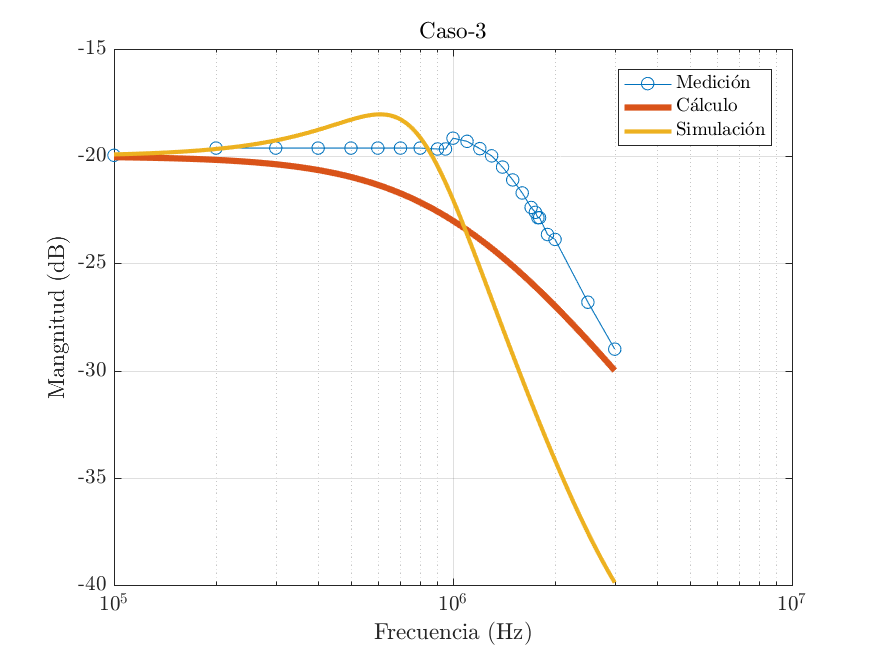
\includegraphics[width=\textwidth]{Caso-3_mag_inv}
\caption{Magnitud}\label{fig=magInvC3}
\end{subfigure}
\begin{subfigure}[http]{0.49\textwidth}
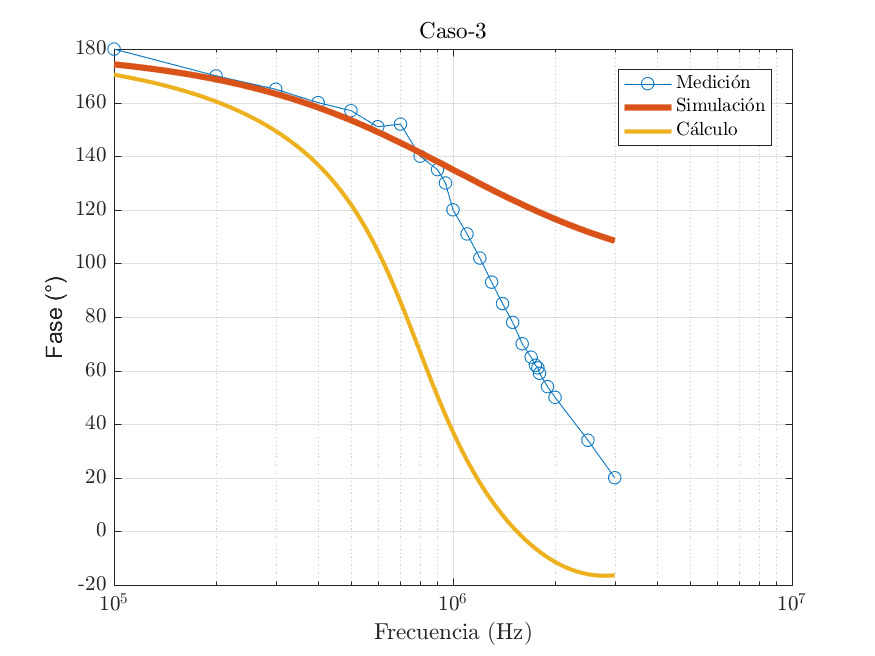
\includegraphics[width=\textwidth]{Caso-3_fase_inv}
\caption{Fase} \label{fig=fasInvC3}
\end{subfigure}
\caption{Caso 3 - superposición respuesta en  frecuencia medida, simulada, calculada}
\end{figure}

En la figura \ref{fig=magInvC3}, se observa un sobrepico, cercano a la frecuencia de corte, en la medicion y la simulacion, sin embargo éste no se observa en los calculos. Suponemos que este fenomeno se deve a la baja ganancia del circuito, lo que amplia su ancho de banda haciendo que el polo domianante del  
$A_{vol}$ se acerque a un polo secundario, provocando el sobrepico.
La diferencia que se observa entre lo simulado y lo medio, se debio a que se tuvo que cambiar de modelo en Ltspice, puesto que el que se utilizo en los otros casos, posee un unico polo del $A_{vol}$ .
Tambien se puede ver el fenomeno de los dos polos, en la fase.Tal como se observa en el grafico \ref{fig=fasInvC3}, la fase medida y simulada varian entre  $180^{\circ}$ y $0^{\circ}$, lo que implica la existencia de dos polos.

\subsubsection{Impedancia de entrada}



\subsubsection{Observaciones del circuito}
Si la $R_{3}$ valiese cero, $V^{+}$ y $V^{-}$, valen lo mismo independientemente de la frecuencia y de la tensión de entrada.De acuerdo a la ecuacion $V_{out}=A_{vol}(V^{+}-V^{-})$, la salida del OpAmp seria cero. Esto mismo se puede ver haciendo el limite tendiendo a cero de $R_{3}$ de la ecuación \ref{eq=poloDominante}, la salida del es cero independientemente de la entrada.
\\
La función de la $R_{4}$ de cargar al circuito, sin embargo no puede tener cualquier valo. Como la salida del circuito tiene una tensión $V_{o}$ independiente de la carga, si se conecta una resistencia de valor pequeño la corriente debería aumentar para así mantener la salida. En principio esa resistencia podría ser tan pequeña como se desee, entonces la corriente debería aumentar para mantener la tensión. Sin embargo los OpAmp reales tienen una máxima corriente de salida $i_{max}$, entonces se debe cumplir $R_{4}> \frac {V_{o}}{ i_{max}}$.




\subsection{Circuito no inversor}


\end{document}
